\pagenumbering{gobble}
\begin{titlingpage}
\thispagestyle{empty}
\newgeometry{left=2.25in,bottom=2in,right=2.25in,top=2.5in}
\begin{centering}
\rule{\textwidth}{1pt}\par
\vspace{0.5\baselineskip}
{\HUGE\scshape State-dependent forces in \\ cold quantum gases\\}
\vspace{\baselineskip}
\rule{\textwidth}{1pt}\par
\vfill
{\Huge Christopher Billington}\\
\vfill
\Large Submitted in total fulfilment of the requirements\\
of the degree of Doctor of Philosophy\\
\vspace{\baselineskip}
\textbf{Supervisory committee:}\\
Prof~Kristian Helmerson\\
Dr~Lincoln Turner\\
Dr~Russell Anderson\\
\vfill
\begin{minipage}{3cm}
\centerfloat

\includegraphics[width=2.5cm]{figures/Monash_crest_A4.pdf}
\end{minipage}\\
{\Large School of Physics and Astronomy\\
Monash University\\
\vspace{\baselineskip}
June, 2018}\\
\end{centering}
% \draftinfo
\restoregeometry
\end{titlingpage}

\pagenumbering{roman}

\cleardoublepage

\vspace*{\fill}

\begin{center}
\begin{minipage}{0.95\textwidth}

\begin{center}
\textit{Copyright Notices}
\end{center}

{\textit{Notice 1}}

Under the Copyright Act 1968, this thesis must be used only under the normal conditions of scholarly fair dealing.
In particular no results or conclusions should be extracted from it, nor should it be copied or closely paraphrased in whole or in part without the written consent of the author.
Proper written acknowledgement should be made for any assistance obtained from this thesis.

\bigskip

{\textit {Notice 2}}

I certify that I have made all reasonable efforts to secure copyright permissions for third-party content included in this thesis and have not knowingly added copyright content to my work without the owner's permission.

\end{minipage}
\end{center}

\vspace*{\fill}
\vspace*{\fill}

\chapter*{Abstract}

Studies in cold quantum gases enjoy a tight coupling between theory and experiment. Bose--Einstein condensates are well modelled by mean-field theory, with which one may efficiently simulate a large number of Bose-condensed atoms. The efficacy and tractability of this and other approximate models make them powerful tools for guiding experiments in cold quantum gases for precision measurement, quantum computation, quantum simulation, and studies of superfluid turbulence.

Whilst mean-field theory well describes the motional state of atoms in a Bose--Einstein condensate, their internal states---the motion of their electrons relative to the nucleus---are instead described by the Schr\"odinger equation. With this equation---reduced to a small discrete basis for only the relevant electronic states of a given problem---modelling the internal state of an atom is also tractable. Above the critical temperature required for condensation, atoms are not condensed, and move through space more like classical billiard balls---no longer described by mean-field theory. If the atoms' residual wavelike behaviour can be ignored---as it often can---their motion can be modelled using classical mechanics even though their internal state is modelled quantum-mechanically. This approach, called a `semiclassical' model, has been used with great success for theoretical studies of laser cooling, and has been used by Christopher Watkins in the Monash Quantum Fluids group in simulations of evaporative cooling in magnetic traps.

However, the fundamental disconnect between quantum mechanics and classical mechanics prevents na\"ive semiclassical models from reproducing one of the bedrock experiments of quantum mechanics---the Stern--Gerlach experiment. In this experiment, the force on atoms depends on their internal state, such that atoms are measured to have probabilistically taken any of a number of trajectories. These trajectories are still individually classical, but cannot be reproduced collectively within the framework of deterministic classical motion. This problem led to an unphysical heating of the atom cloud in the aforementioned simulations of evaporative cooling, due to the sensitivity of Majorana losses on the details of Stern--Gerlach separation of atoms near the magnetic field zero of the trap.

In this thesis I develop a method to resolve this disconnect to allow semiclassical models to include state-dependent forces. The method makes use of \emph{hidden variables}---labels carried alongside quantum states that declare in some sense what state the system is `really' in, when the quantum description of the state is that of a superposition. Although



\chapter*{Declaration}

This thesis contains no material that has been accepted for the award of any other degree or diploma in any university or other institution. To the best of my knowledge the thesis contains no material previously published or written by another person, except where due reference is made in the text of the thesis. For parts of this thesis that are based on joint research or publications, the relative contributions of the respective authors are detailed appropriately.

\begin{center}
\vspace{1.5cm}
\rule{8cm}{1pt}\\
\raisebox{0.5cm}[0pt][0pt]{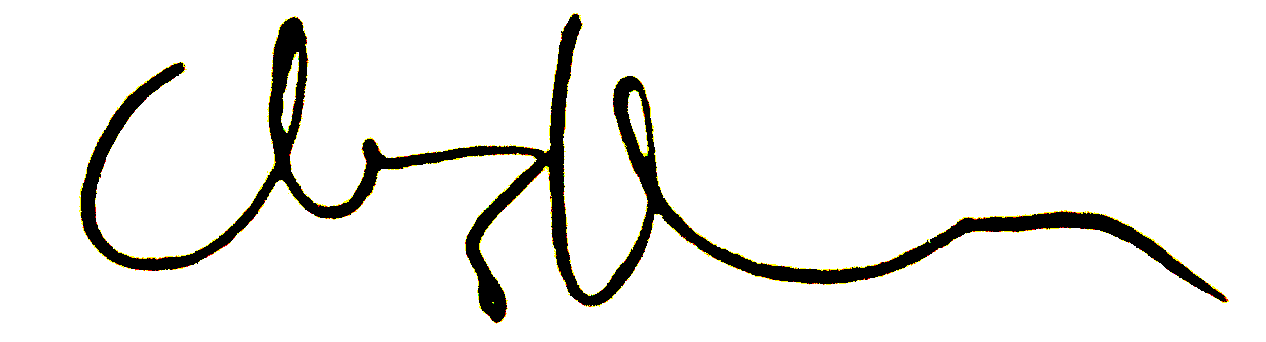
\includegraphics[scale=0.1]{submission/cjb}}\\
Christopher Billington

\vspace{1.5cm}
\rule{8cm}{1pt}\\
\raisebox{0.5cm}[0pt][0pt]{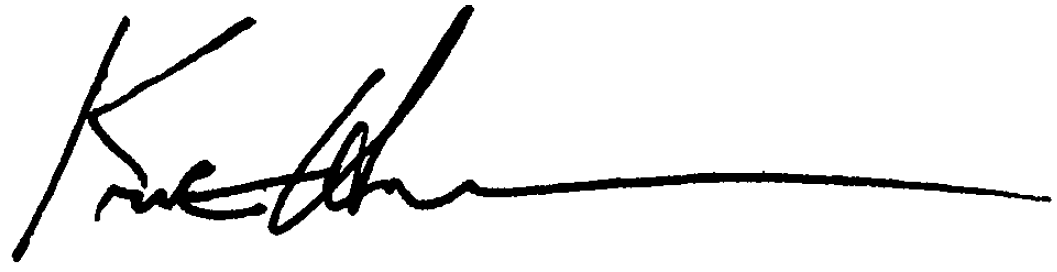
\includegraphics[scale=0.15]{submission/kh}}\\
Professor Kristian Helmerson  

\vspace{1.5cm}
\rule{8cm}{1pt}\\
\raisebox{0.6cm}[0pt][0pt]{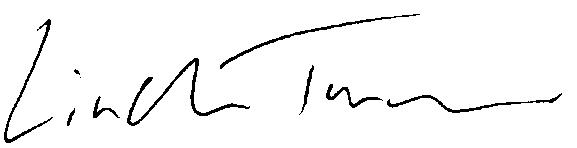
\includegraphics[scale=0.9]{submission/ldt}}\\
Dr Lincoln Turner

\vspace{1.5cm}
\rule{8cm}{1pt}\\
\raisebox{0.5cm}[0pt][0pt]{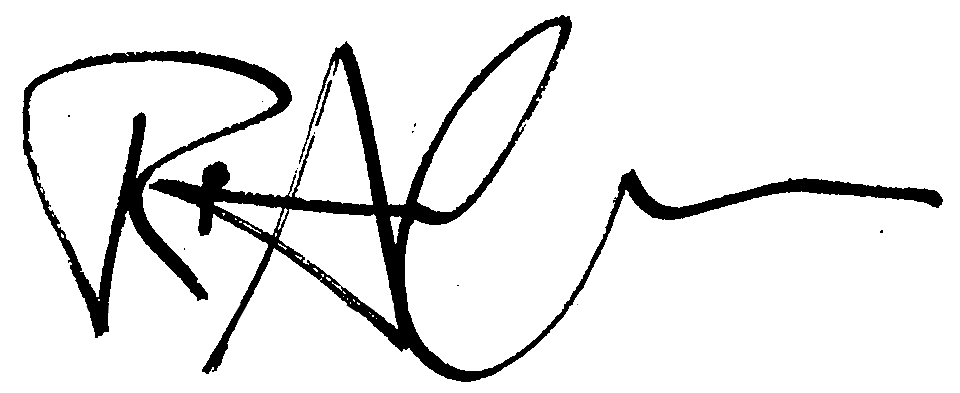
\includegraphics[scale=0.1]{submission/rpa}}\\
Dr Russell Anderson 

\end{center}

\chapter*{Acknowledgements}

% Over the past few years during my PhD, I've been able to learn fascinating things from interesting people, play with fun technological toys, and contribute meaningfully to scientific progress. I could not have done any of this without the support, friendship, and mentorship of many people. The Science Advanced cohort w Lincoln Turner brought me up to speed on a wide range of topics

\cleardoublepage

\tableofcontents
% \listoffigures
% \listoftables
\cleardoublepage
\pagenumbering{arabic}
